% !Mode:: "TeX:UTF-8"

\chapter{绪论}
\section{研究背景与课题来源}
\subsection{研究背景}

自有建筑XXXXX~\cite{PLC2006DXTYG,SGR2012TYCG}和大XXX题~\cite{jones2011cocktail,pick1989inhibiting}。

XXXXX


\subsection{课题来源}
本研究是国家自然科学基金面上项目《特大空间中声XXX》(基金编号51XXX)的组成部分之一。
%因盲审需要,此处暂空。
\section{概念解释}

\textbf{特XXXX:}
XXX)。

\section{国内外研究综述}
\subsection{国外研究综述}

国外针对特大XXX

\textbf{一、特大空间声XXX究}

XXXX。

\textbf{(1)大XXX}

XXX



\subsection{国内研究综述}

国内对XXX。

\subsection{研究综述总结与问题的提出}

通过上述XXXX研究。

\section{研究目的与意义}
\subsection{研究目的}

本文的研究目的为:

(1)XXX;

(2)XXX;

(3)XXX;

(4)XXX。


\subsection{研究意义}

本文X
(1)理论研究意义。

XXX

(2)社会经济意义

XXX。


\section{研究内容及研究方法}
\subsection{研究方法}

XXXX




\subsection{研究框架}
对于XXX。

\begin{figure}[b]
\centering
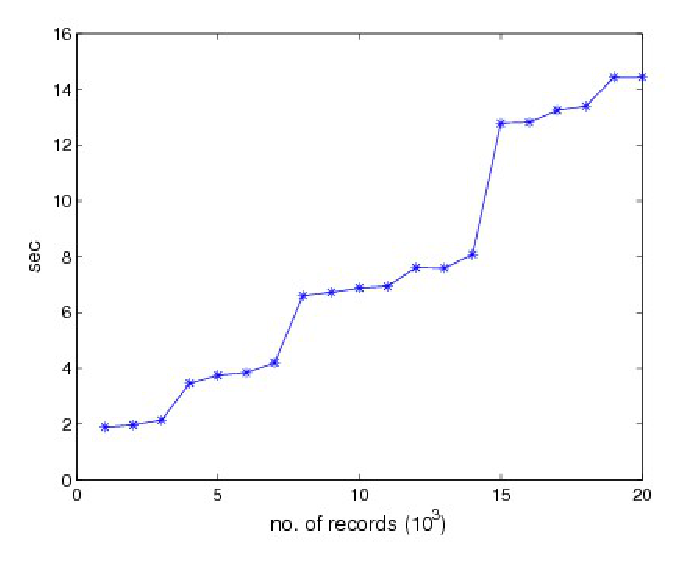
\includegraphics[width=0.98\textwidth]{phd_figures/dataSize.eps}
\caption{论文框架与技术路线,作者自绘。}\label{fig:Chapter1-lilun-kuangjia}
\vspace{\baselineskip} %表示图与正文空一行
\end{figure}

\subsection{创新点}

本研XXXX。







